\section{Country Avoidability}
\label{avoid_results}

\subsection{Avoidability Metrics}
\label{metrics}
We introduce a new metric and algorithm to measure how often a client in Country X can avoid a specified Country Y.  Using the proposed metric and algorithm, we can compare how well the different methods achieve country avoidance for a specified client Country X and unfavorable Country Y.

{\bf Avoidability Metric.}  This metric quantifies how often traffic can avoid Country Y when it originates in Country X.  Avoidability is explained as the fraction of paths that start in Country X and do not transit Country Y; more formally:

\[Avoidability(X,Y) = \frac{paths_{X,\bcancel{Y}}}{paths_{X}}\]

where $paths_{\bcancel{Y}}$ represent the paths from Country X that do not pass through Country Y, and $paths_{X}$ represent all paths that originate from Country X. The resulting value will be in the range [0,1], where 0 means the country is unavoidable for all of the domains in our study, and 1 means the client can avoid Country Y for all domains in our study.  This metric is used on country-level paths calculated during the measurements in Section~\ref{pipeline}.

{\bf Avoidability Algorithm with Relays.}  Measuring the avoidability of a country Y from a client in Country X using relays has two components: 1) is Country Y on the path from the client in Country X to the relay?  2) is Country Y on the path from the relay to the domain?  For every domain, our algorithm checks if there exists at least one path from the client Country X through any relay and on to the domain, and does not transit Country Y.  The psuedo-code for the algorithm is shown in Algorithm~\ref{avoid_algo}.

\begin{algorithm}
\caption{Avoidability Algorithm}
\label{avoid_algo}
\begin{algorithmic}[1]
\Function{CalcAvoidance}{set $paths1$, set $paths2$, string c}
    \State set $usableRelays$
    \For{each $(relay,path)$ in $paths1$} 
    	\If{$c$ not in $path$}
		\State $usableRelays \gets path$
	\EndIf
    \EndFor
    \State set $accessibleDomains$
    \For{each $(relay,domain,path$ in $paths2$}
    \If{$relay$ in $usableRelays$}
        \If{$c$ not in $path$}
        \State $accessibleDomains \gets domain$
        \EndIf
    \EndIf
    \EndFor
    \State $D \gets$ number of all unique domains in $paths2$
    \State $A \gets$ length of $accessibleDomains$
    \State \Return $A / D$
\EndFunction
\end{algorithmic}
\end{algorithm}

The output of the algorithm is a value in the range [0,1] that can be compared to the output of the Avoidability Metric described above.  

{\bf Upperbound on Avoidability.}  While the Avoidability metric and algorithm provide a method to quantify how avoidable Country Y is from a client in Country X, it may be the case that a number of domains are hosted in Country Y, so the Avoidance value for these countries would never reach 1.0.  For this reason, we measured the upperbound on avoidance for given pair of (Country X, Country Y) that represents the best case value for avoidance.  The pseudocode for the algorithm is shown in Algorithm \ref{upperbound_algo}.

\begin{algorithm}
\caption{Avoidance Upperbound Algorithm}
\label{upperbound_algo}
\begin{algorithmic}[1]
\Function{CalcUpperbound}{set $relayDomainPaths$, string $c$}
    \State $zeros(domainLocations)$
    \For{each $(r,d,p)$ in $relayDomainPaths$} 
		\State $dest \gets $ last item in $p$
		\State $domainLocations[d] \gets dest$
    \EndFor
    \State set $accessibleDomains$
    \For{each $domain$ in $domainLocations$}
    \If{$domainLocations[domain] \neq $ set[$c$]}
    \State $accessibleDomains \gets domain$
    \EndIf
    \EndFor
    \State $D \gets$ all unique domains in  $relayDomainPaths$
    \State $A \gets$ length of $accessibleDomains$
    \State \Return $A / D$
\EndFunction
\end{algorithmic}
\end{algorithm}

The algorithm analyzes the destinations of all domains from all relays and if there exists at least one destination for a domain that is not in Country Y, then this increases the upperbound value.  An upperbound value of 1.0 means that every domain studied is hosted (or has a replica) outside of Country Y.  This value puts the Avoidance values in perspective for each (Country X, Country Y) pair. 

After applying the metrics described in Section \ref{metrics} to country-level paths, we compared how avoidable different countries could be when using open resolvers or relays to how often traffic currently transits those countries.  First, we discuss how effective open resolvers are at country avoidance.  Then we show how effective relays are at country avoidance and at keeping local traffic local.  Avoidance values are shown in Table \ref{tab:avoid}.

\begin{table*}[t]
\centering
\begin{tabular}{|P{25mm}|cc|cc|cc|cc|cc|}
\multicolumn{1}{l}{}    & \headrow{No Relay} & \headrow{Relays} & \headrow{No Relay} & \headrow{Relays} & \headrow{No Relay} & \headrow{Relays}   & \headrow{No Relay} & \headrow{Relays}  & \headrow{No Relay} & \headrow{Relays} \\\hline
\textit{Country}    &\multicolumn{2}{c|}{\textit{Brazil}}   &\multicolumn{2}{c|}{\textit{Netherlands}}   &\multicolumn{2}{c|}{\textit{India}} &\multicolumn{2}{c|}{\textit{Kenya}} &\multicolumn{2}{c|}{\textit{United States}}\\
\hline\hline
Brazil               &0.00     &0.00     &1.00  &1.00   &1.00    &1.00  &1.00   &1.00  &1.00  &1.00  \\\hline\hline
Canada               &.987     &1.00     &.993  &1.00   &.984    &.980  &.992   &.996  &.919  &1.00  \\\hline
United States        &.156     &.626     &.417  &.630   &.285    &.656  &.384   &.400  &0.00  &0.00  \\\hline\hline
France               &.941     &1.00     &.898  &.996   &.896    &1.00  &.779   &.989  &.896  &.997  \\\hline
Germany              &.995     &1.00     &.950  &.996   &.968    &.994  &.952   &1.00  &.992  &1.00  \\\hline
Great Britain        &.976     &1.00     &.860  &.996   &.796    &1.00  &.500   &.979  &.994  &1.00  \\\hline
Ireland              &.972     &.992     &.894  &.996   &.969    &.994  &.867   &.993  &.994  &.997  \\\hline
Netherlands          &.981     &.996     &0.00  &0.00   &.879    &.997  &.747   &.996  &.969  &.997  \\\hline
Spain                &.824     &1.00     &.996  &.996   &1.00    &1.00  &1.00   &1.00  &1.00  &1.00  \\\hline\hline
Kenya                &1.00     &1.00     &1.00  &1.00   &1.00    &1.00  &0.00   &0.00  &1.00  &1.00  \\\hline
Mauritius            &1.00     &1.00     &1.00  &1.00   &1.00    &1.00  &.678   &.996  &1.00  &1.00  \\\hline
South Africa         &1.00     &1.00     &1.00  &1.00   &1.00    &1.00  &.666   &.666  &1.00  &1.00  \\\hline\hline
United Arab Emirates &1.00     &1.00     &1.00  &1.00   &1.00    &1.00  &.848   &.996  &1.00  &1.00  \\\hline
India                &1.00     &1.00     &.993  &1.00   &0.00    &0.00  &.942   &1.00  &.999  &1.00  \\\hline
Singapore            &.999     &1.00     &.998  &1.00   &.730    &.949  &.960   &1.00  &.997  &1.00  \\\hline
\end{tabular}
\caption{Avoidance values for differing techniques of country avoidance.}
\label{tab:avoid}
\end{table*}

\subsection{Avoidance with Open Resolvers}
\annie{This is still being calculated, but I'll update as soon as possible.}

\subsection{Avoidance with Relays}
As seen in Table \ref{tab:avoid}, there are two significant trends: 1) the ability for a client to avoid a given Country Y increases with the use of relays, and 2) the least avoidable countries are surveillance states.

\subsubsection{Avoidance Increases with Relays}
In almost every (Country X, Country Y) pair, where Country X is the client's country (Brazil, Netherlands, India, Kenya, or the United States) and Country Y is the country to avoid, the use of an overlay network makes Country Y more avoidable than the current default routes.  The one exception we encountered is when a client is located in Kenya and wants to avoid South Africa; South Africa is on the path between the client and every relay, and therefore the client should not use the relays.  

\begin{figure}
\centering
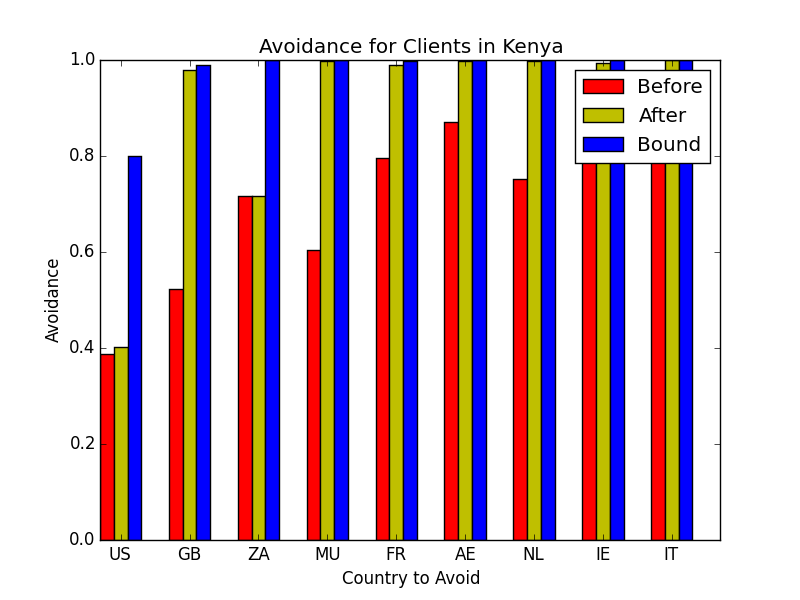
\includegraphics[width=.5\textwidth]{ke_avoidance}
\caption{Avoidance values for Kenyan clients without relays, with relays, and the upperbound.}
\label{fig:ke_avoidance}
\end{figure}

{\bf For 84\% of the (Country X, Country Y) pairs shown in Table \ref{tab:avoid} the avoidance with relays reaches the upperbound on avoidance.}  (Kenya, Country Y) pairs have the lowest percentage of avoidance values that reach the upperbound, showing that it is more difficult for Kenyan clients to avoid a given country.  This is not to say that relays are not effective for clients in Kenya; for example, the default routes to the top 100 domains for Kenyans avoid Great Britain 50\% of the time, but with relays this percentage increases to about 98\% of the time, and the upper bound is about 98\%. Figure \ref{fig:ke_avoidance} shows default avoidance, avoidance with relays, and the upperbound for Kenya; it's clear that despite having the worst position for avoidance out of the studied countries, in most cases the avoidance with relays either reaches or because extremely close to the upperbound.  {\bf The highest percentage (100\%) of avoidance values that reach the upperbound are for clients in the United States} -- relays help clients in this country avoid all other Country Y in all cases that the domain is not hosted in Country Y.  

\subsubsection{Surveillance States are the Least \\Avoidable}
Certain surveillance states discussed in Section \ref{surv} are completely unavoidable a small fraction of time from certain client locations.  France is unavoidable a for a small percentage of domains for clients located in the Netherlands, Kenya, and the United States.  Similarly, clients in the Netherlands and Kenya cannot avoid Great Britain for a small fraction of domains.  

{\bf Avoidance values for (Country X, United States) pairs are significantly lower than any other Country Y for all three situations: without relays, with relays, and the upperbound.}   Despite increasing clients' ability to avoid the United States, relays are not as effective at helping clients avoid this country as compared to the effectiveness of the relays at avoiding all other Country Y.  Clients in India can avoid the United States more often than clients in Brazil, Netherlands, and Kenya, with an avoidance value of .656 when using relays.  Kenyan clients can only avoid the United States 40\% of the time even while using relays.  Additionally, the upperbound for avoiding the United States is significantly lower in comparison to any other country.  

\subsection{Keeping Local Traffic Local}
For the cases where there were relays located in one of the five studied countries, we evaluated how effectively the use of relays kept local traffic local.  This evaluation was possible for Brazil and the United States.  In both cases, we found the percentage of tromboning traffic decrease, and the number of countries that traffic tromboned to decreased.  Tromboning Brazilian traffic decreased from 13.2\% without relays to 9.7\% with relays; when relays are used, all tromboning traffic goes only to the United States.  With the use of relays, there was only 1.3\% tromboning traffic for a United States client, whereas without relays there was 11.2\% tromboning traffic.  For the 1.2\% of traffic that trombones from the United States, it all goes only to Ireland.
